
\documentclass[12pt]{article}

\begin{document}

% Additional packages
\usepackage[main=english,slovak]{babel}
% For thesis written in English just change the order of languages:
% \usepackage[main=english,slovak]{babel}

\usepackage{listings}  % for source code
% Listings settings
% See for details: https://en.wikibooks.org/wiki/LaTeX/Source_Code_Listings
\usepackage{qtree}
\usepackage{tikz-qtree}
\usepackage{graphicx}
\usepackage{subcaption}

\lstset{
    basicstyle=\small\ttfamily,  % smaller typewriter font
    showstringspaces=false       % don't show spaces in string
}

% Location of file with bibliography resources
\addbibresource{chapters/bibliography.bib}

Technical University of Košice

Faculty of Mining, Ecology, Process Control 
and Geotechnologies

Student Scientific Conference




Section S2A Control and Logistics




Automatický tvorca predikčných modelov

Automatic prediction model builder

Name and surname, degree: Ales Jandera (Bc.)
Level of study: II. - Master degree
Year of study: 2.
Study programme: Process control of raw materials extraction and processing 
Supervisor of the work: doc. Ing. Tomas Skovranek, Phd.

ABSTRAKT
Text in the mother tongue.
Lorem ipsum dolor sit amet, consectetuer adipiscing elit. Praesent id justo in neque elementum ultrices. Morbi leo mi, nonummy eget tristique non, rhoncus non leo. Phasellus enim erat, vestibulum vel, aliquam a, posuere eu, velit. Aliquam id dolor. Ut enim ad minima veniam, quis nostrum exercitationem ullam corporis suscipit laboriosam, nisi ut aliquid ex ea commodi consequatur? Praesent dapibus. Nullam faucibus mi quis velit. Phasellus faucibus molestie nisl. Suspendisse sagittis ultrices augue. Aliquam erat volutpat. Maecenas aliquet accumsan leo. Integer tempor. Cras elementum. Cum sociis natoque penatibus et magnis dis parturient montes, nascetur ridiculus mus. Suspendisse sagittis ultrices augue. Donec quis nibh at felis congue commodo. Curabitur ligula sapien, pulvinar a vestibulum quis, facilisis vel sapien.
Kľúčové slova: 
ABSTRACT
Text in the English language
Lorem ipsum dolor sit amet, consectetuer adipiscing elit. Praesent id justo in neque elementum ultrices. Morbi leo mi, nonummy eget tristique non, rhoncus non leo. Phasellus enim erat, vestibulum vel, aliquam a, posuere eu, velit. Aliquam id dolor. Ut enim ad minima veniam, quis nostrum exercitationem ullam corporis suscipit laboriosam, nisi ut aliquid ex ea commodi consequatur? Praesent dapibus. Nullam faucibus mi quis velit. Phasellus faucibus molestie nisl. Suspendisse sagittis ultrices augue. Aliquam erat volutpat. Maecenas aliquet accumsan leo. Integer tempor. Cras elementum. Cum sociis natoque penatibus et magnis dis parturient montes, nascetur ridiculus mus. Suspendisse sagittis ultrices augue. Donec quis nibh at felis congue commodo. Curabitur ligula sapien, pulvinar a vestibulum quis, facilisis vel sapien.
Keywords:


    \chapter{Analysis}\label{analysis}
      \section{Prediction mathematical models}
      Mathematical prediction models are tools used to forecast the behavior of a system or process. They are typically built using mathematical equations or algorithms that are designed to describe the relationship between the input and output variables of the system.\\
    \\
    There are several types of mathematical prediction models, including linear regression, time series analysis, and machine learning algorithms such as neural networks and decision trees. Each type of model has its strengths and weaknesses, and the choice of model depends on the specific problem being addressed.\\
    \\
    Linear regression models are used to describe the relationship between two or more variables by fitting a straight line to the data. Time series analysis is used to predict future values of a variable based on its past values, and can be used to forecast trends, seasonal patterns, and other patterns in time series data.\\
    \\
    Machine learning algorithms are increasingly being used for prediction modeling, as they can learn complex relationships between input and output variables and adapt to changing data patterns. Neural networks, for example, are designed to simulate the structure and function of the human brain and can be used for tasks such as image recognition, natural language processing, and predicting the outcome of events.\\
    \\
    Mathematical prediction models are used in a wide range of fields, including finance, economics, engineering, and the natural sciences. They can be used to forecast stock prices, predict the spread of disease, optimize industrial processes, and much more.
      \subsection{Regresion models}
      Regression models are a~type of statistical models used to examine the~relationship between a~dependent variable
and one or more independent variables~\cite{Fahrmeir}.
The goal of regression analysis is to model the~relationship between these variables and make predictions about
the dependent variable based on the~values of the~independent variables. Regression models are widely used in many
fields, including economics, finance, marketing, and social sciences, to make predictions and understand the
relationship between variables. There are several types of regression models, including:
\begin{itemize}
    \item Linear regression is a~simple regression model where the~relationship between the~dependent and independent variables is modeled using a~linear equation.
    \item Logistic regression is used for binary classification problems where the~dependent variable is binary and the~goal is to model the~relationship between the~independent variables and the~probability of the~dependent
    variable being either 0 or 1.
    \item Multiple regression is used when there are multiple independent variables and the~goal is to model the
    relationship between all of these variables and the~dependent variable.
    \item Polynomial regression is used when the~relationship between the~dependent and independent variables
    is non-linear and can be modeled using a~polynomial equation.
\end{itemize}

The choice of regression model depends on the~nature of the~data and the~research question being asked.
      \subsection{Time-series models}
      Time-series models are mathematical models used to analyze and forecast data that are collected over time~\cite{Cryer}. These models are used to study and make predictions about the~trends, patterns, and behavior of the~data over time, taking into account historical values and their relationship with the~present. Time-series models are widely used in areas such as economics, finance, and weather forecasting, among others. The~models are based on various statistical techniques, including ARIMA (AutoRegressive Integrated Moving Average), SARIMA (Seasonal ARIMA), and exponential smoothing, among others. The~goal of time-series modeling is to build a~mathematical representation of the~underlying process that generates the~time-series data, allowing for accurate prediction of future values. Time-series models are statistical models used to analyze and make predictions about time-dependent data. They are widely used in various fields, including finance, economics, engineering, and social sciences.\\
    \\
    Time-series models make use of past values of a~variable to predict future values.
They assume that there is a~pattern or trend in the~data that can be used to forecast future behavior.
Some commonly used time-series models include:
    \begin{itemize}
        \item Autoregressive Integrated Moving Average (ARIMA). This model is used to analyze and forecast stationary
        time-series data. It consists of three components: autoregression, differencing, and moving average.
        \item Seasonal Autoregressive Integrated Moving Average (SARIMA) is~an~extension of ARIMA
        that takes into account seasonal patterns in the~data.
        \item Exponential Smoothing (ETS) is used to forecast time-series data that has a~trend
        and/or seasonality. It uses a~smoothing parameter to assign more or less weight to past observations
        based on their recency.
        \item Vector Autoregression (VAR) is used when there are multiple time-series variables
        that influence each other. It can be used to analyze the~relationships between these variables and to make
        predictions about their future be   havior.
        \item These models are valuable tools for analyzing and predicting time-series data, but they require careful
        consideration of the~specific characteristics of the~data being analyzed and the~appropriate model to use.
    \end{itemize}

    Machine learning models are a~subset of artificial intelligence that allows computers to learn and make
predictions or decisions without being explicitly programmed. Machine learning models are based on algorithms
that use statistical methods to find patterns in data and make predictions about new, unseen data.\\
    \\
    There are several types of machine learning models, including \textbf{Supervised learning} where the~model is trained on labeled data, with the~goal of learning the~relationship between the~input features and the~target variable, and making predictions about the~target variable for new, unseen data.
\textbf{Unsupervised learning} where the~model is trained on unlabeled data, with the~goal of finding patterns or structure in the~data, such as clustering or dimensionality reduction. \textbf{Reinforcement learning} where the~model learns by receiving rewards or penalties for its actions in~an~environment, with the~goal of maximizing the~reward over time. \textbf{Deep learning} a~subset of machine learning that uses artificial neural networks with multiple hidden layers to model complex relationships in the~data.\\
    \\
    The choice of machine learning model depends on the~problem being solved and the~type of data being used. Machine learning models have been applied to a~wide range of tasks, including image and speech recognition, natural language processing, and predictive modeling. Advances in machine learning (ML), faster processors and the~availability of digitized healthcare data have contributed to a~growing number of papers describing ML applications in healthcare~\cite{Chen}.\\
    \\
    \noindent \textbf{K-Nearest Neighbors (KNN)} \label{sec:knn}\\
    Machine learning algorithms, K-Nearest Neighbors (KNN), is a~type of artificial intelligence that allows
computers to learn and make decisions based on data. KNN is a~simple yet effective algorithm used for
classification and regression tasks in supervised learning.\\
    \\
    KNN is a~non-parametric algorithm, which means it doesn't make any assumptions about the~underlying
distribution of the~data. Instead, it uses the~similarity between data points to classify or predict the~target
variable. The~algorithm works by finding the~k-nearest neighbors to a~new data point and then assigning the~class
label of the~majority of those neighbors to the~new data point.\\
    \\
    For example, if we have a~dataset of images with labels indicating whether each image contains a~cat or a~dog, we can use KNN to classify a~new image by finding the~k-nearest neighbors to the~new image and assigning the label of the~majority of those neighbors to the~new image.\\
    \\
    KNN is a~relatively simple algorithm, but it can be very effective when applied to the~right problems.
It is particularly useful in cases where the~decision boundary is nonlinear or where there is no clear
separation between classes. However, KNN can be computationally expensive when working with large datasets, and
it may not perform well in high-dimensional spaces.

    \section{Neural networks} \label{sec:nn}
    A neural network is a~type of machine learning algorithm inspired by the~structure and function of biological neurons in the~human brain. It is composed of interconnected nodes, called neurons, that are organized into layers. The~input layer receives raw data, such as images or text, and passes it on to the~hidden layers, which perform calculations and apply weights to the~input data to create a~prediction. Finally, the~output layer produces the~final prediction or classification.\\
    \\
    As we can see on image \ref{fig:perceptron} each input $X_n$ should be properly weighted by a~certain weight $W_n$ before all the~signals enter the~summation stage. Afterwards, the~weighted summation is forwarded into the~activation unit producing the~neuron’s output signal.
    \begin{center}
        \begin{figure}[!ht]
            \centering
            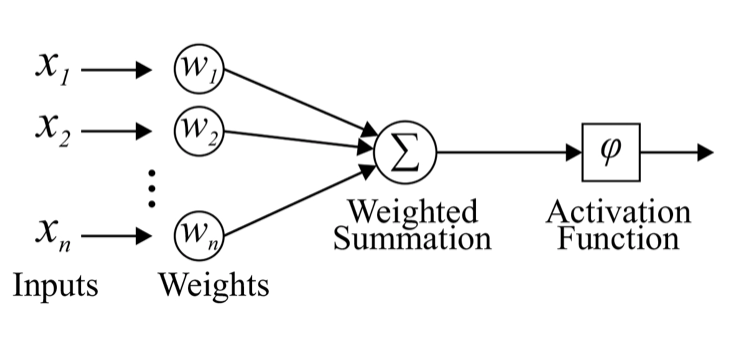
\includegraphics[width=0.6\textwidth]{figures/nn}
            \caption{Perceptron preview. \cite{Mourgias-Alexandris:19}}
            \label{fig:perceptron}
        \end{figure}
    \end{center}
    Neural networks are trained on large datasets using a~process called backpropagation, which adjusts the~weights and biases of the~neurons to minimize the~error between the~predicted output and the~actual output. Once a~neural network has been trained, it can be used to make predictions on new data.\\
    \\
    A neuron is a~basic building block of a~neural network, also known as~an~artificial neuron or a~perceptron.
It is modeled after the~biological neuron in the~human brain, which receives input signals from other neurons,
processes them, and sends output signals to other neurons.\\
    \\
    In a~neural network, a~neuron receives input from other neurons or directly from the~input data, applies a~mathematical function to the~input, and produces~an~output that is sent to other neurons in the~network. The~input to a~neuron is usually a~vector of numbers, and each input is multiplied by a~corresponding weight. The~neuron then sums up the weighted inputs, adds a~bias term, and applies~an~activation function to the~result.\\
    \\
    The purpose of the~activation function is to introduce nonlinearity into the~neuron, which allows the~neural network to learn complex patterns and relationships in the~data. There are several different types of activation functions that can be used, such as the~sigmoid function, ReLU (Rectified Linear Unit) function, and tanh (hyperbolic tangent) function.\\
    \\
    The output of a~neuron is typically fed into other neurons in the~next layer of the~neural network. The~weights and biases of the~neurons are adjusted during the~training process using a~technique called backpropagation, which involves computing the~gradient of the~error with respect to the~weights and updating them using~an~optimization algorithm such as stochastic gradient descent.\\
    \\
    Overall, the~neurons in a~neural network work together to learn patterns and relationships in the~input data and produce output that can be used for a~variety of tasks, such as classification, regression, and prediction.\\
Neural networks have been successfully applied in a~wide range of fields, including image and speech recognition, natural language processing, and autonomous vehicles, among others. Neural networks can be broadly classified into the~following types:\\
    \\
    \textbf{Feedforward Neural Networks}\\
    These are the~most basic type of neural networks, where the~information flows only in one direction,from input to output. These networks can have one or more hidden layers and are often used for classification or regression tasks. Shema on basic feedforward NN is on fig~\ref{fig:ff}
    \begin{center}
        \begin{figure}[!ht]
            \centering
            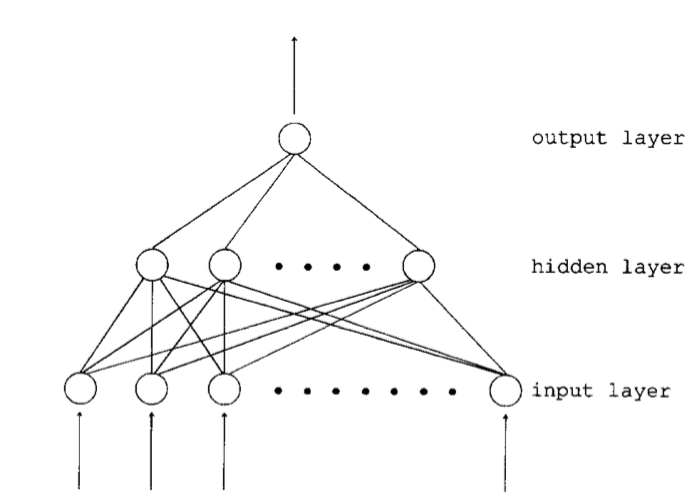
\includegraphics[width=0.6\textwidth]{figures/ff}
            \caption{Typical feed-forward neural network composed of three layers. \cite{svozil1997quantum}}
            \label{fig:ff}
        \end{figure}
    \end{center}
    \textbf{Convolutional Neural Networks (CNNs)}\\
    These networks are specialized for processing images and are commonly used in computer vision tasks. They use convolutional layers to extract features from images and can learn to recognize patterns and objects in images see in fig~\ref{fig:cn}
    \begin{center}
        \begin{figure}[!ht]
            \centering
            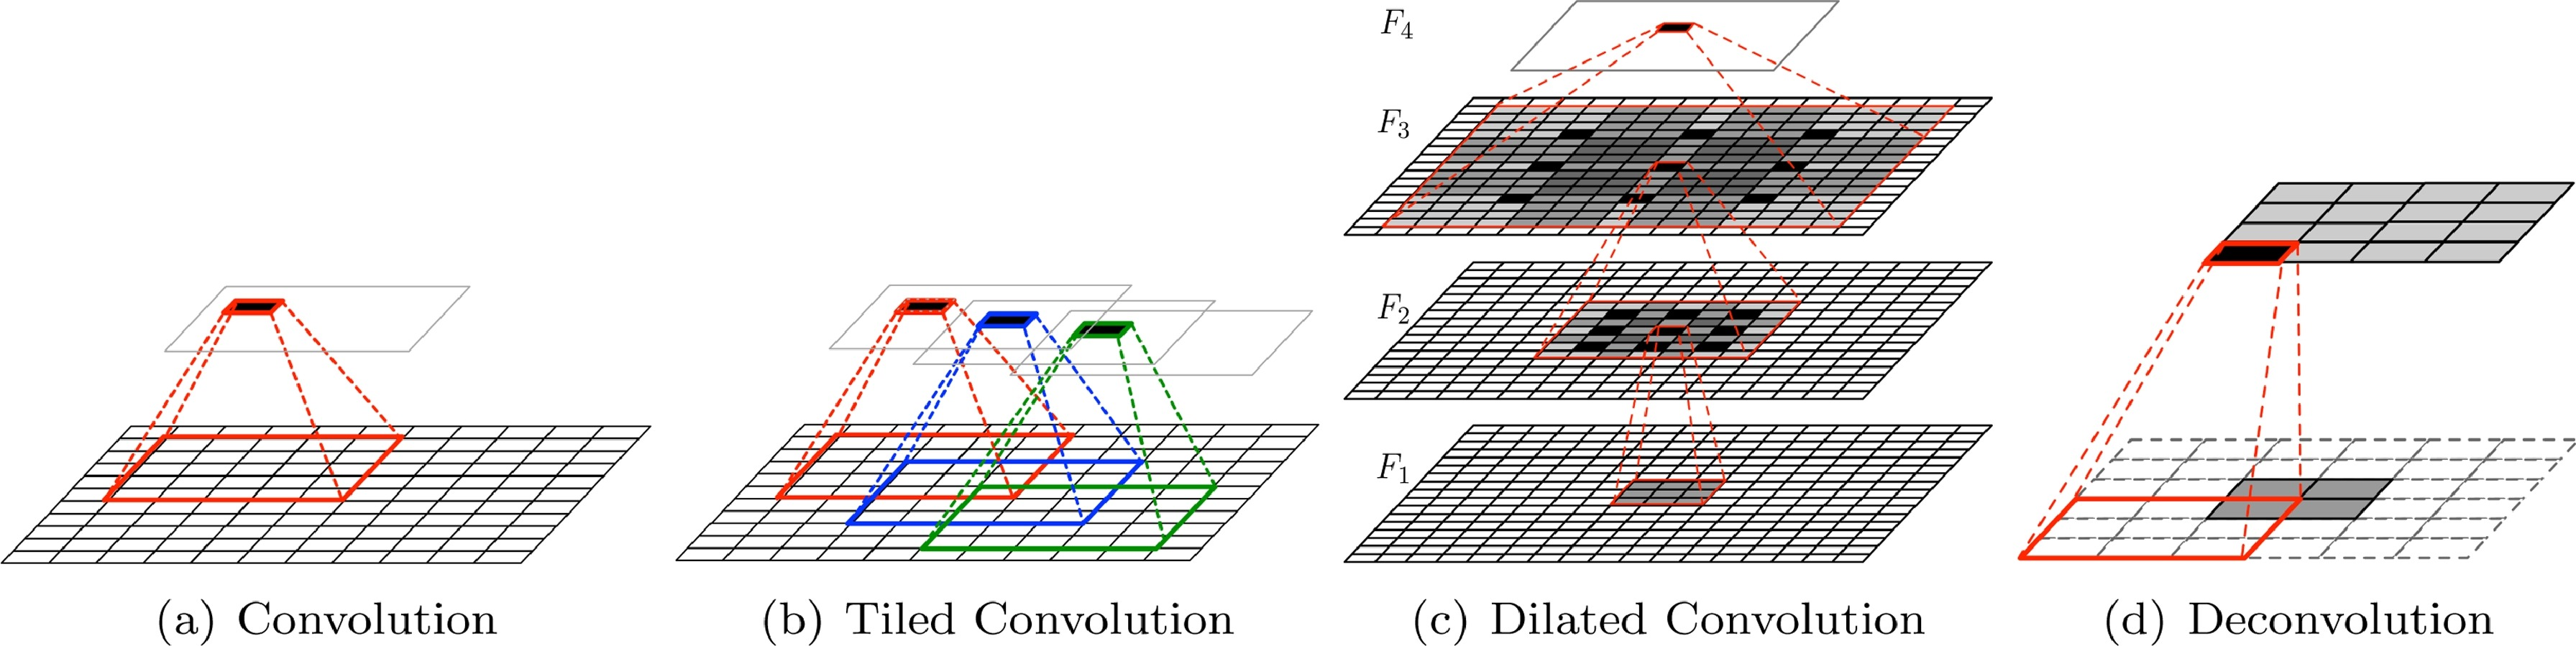
\includegraphics[width=0.8\textwidth]{figures/cn}
            \caption{Illustration of (a) Convolution, (b) Tiled Convolution, (c) Dilated Convolution, and (d)
                Deconvolution. \cite{GU2018354}}
            \label{fig:cn}
        \end{figure}
    \end{center}
    \textbf{Recurrent Neural Networks (RNNs)}\\
    These networks are designed to work with sequential data, such as time-series or natural language data. They have loops that allow information to be passed from one time-step to the~next, enabling them to capture temporal dependencies in the~data, described on fig~\ref{fig:rn}
    \begin{center}
        \begin{figure}[!ht]
            \centering
            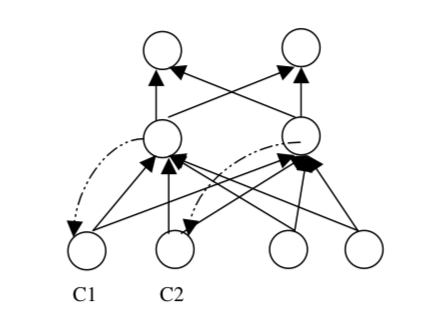
\includegraphics[width=0.4\textwidth]{figures/rn}
            \caption{Typical recurrent network. \cite{medsker2001recurrent}}
            \label{fig:rn}
        \end{figure}
    \end{center}
    \textbf{Long Short-Term Memory Networks (LSTMs)}\\
    These are a~type of RNN that are designed to address the~problem of vanishing gradients in traditional RNNs. They use memory cells and gates to selectively retain or forget information over time, making them well-suited for learning from long sequences. As you can see on fig~\ref{fig:ltmn} color indicates degree of memory activation.
    \begin{center}
        \begin{figure}[!ht]
            \centering
            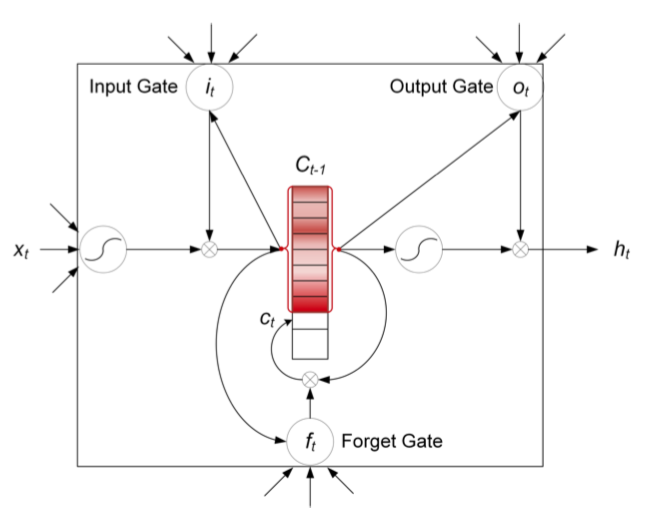
\includegraphics[width=0.35\textwidth]{figures/ltmn}
            \caption{Long short-term memory network. \cite{cheng2016long}}
            \label{fig:ltmn}
        \end{figure}
    \end{center}
    \textbf{Autoencoder Neural Networks}\\
    These networks are used for unsupervised learning and are designed to learn a~compressed representation of the~input data. As we can see on figure~\ref{fig:ann} they consist of~an~encoder that maps the~input data to a~compressed representation, and a~decoder that maps the~compressed representation back to the~original data.
    \begin{center}
        \begin{figure}[!ht]
            \centering
            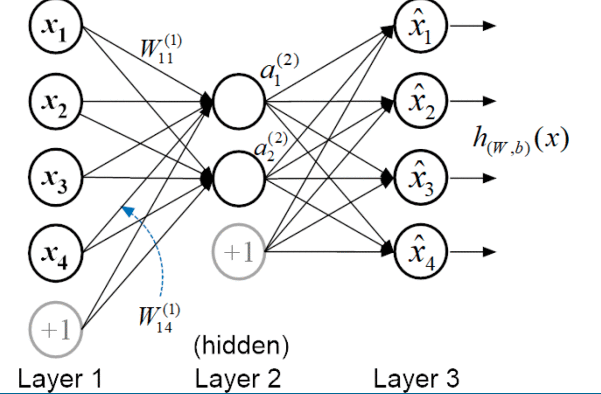
\includegraphics[width=0.5\textwidth]{figures/ann}
            \caption{An autoencoder neural network. \cite{luo2018distributed}}
            \label{fig:ann}
        \end{figure}
    \end{center}
    \textbf{Generative Adversarial Networks (GANs)}\\
    These networks consist of two networks, a~generator and a~discriminator (see on figure~\ref{fig:gan}), that are trained together in a~game-theoretic framework. The~generator is trained to generate realistic data samples, while the~discriminator is trained to distinguish between real and generated data samples.
    \begin{center}
        \begin{figure}[!ht]
            \centering
            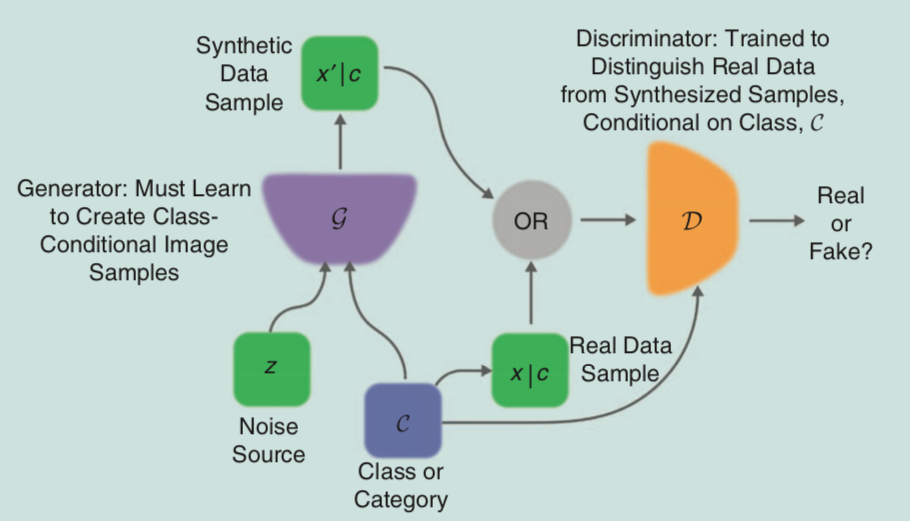
\includegraphics[width=0.5\textwidth]{figures/gan}
            \caption{The conditional GAN schema. \cite{creswell2018generative}}
            \label{fig:gan}
        \end{figure}
    \end{center}

    These are some of the~most common types of neural networks, but there are many other specialized types of neural networks that have been developed for specific tasks, such as object detection, speech recognition, and
natural language processing.\\

    \subsection{Classification} \label{subsec:clasification}
    Neural network data classification is a~technique for categorizing data into different classes or categories based on patterns and features present in the~data. a~neural network is a~type of machine learning algorithm that is modeled after the~structure and function of the~human brain. It is composed of interconnected nodes or neurons that are organized into layers.\\
    \\
    In a~classification task, the~neural network is trained on a~dataset that is labeled with the~correct
class for each example. During training, the~network learns to recognize patterns and features in the~input data
that are associated with each class. The~process of training involves adjusting the~weights and biases of the~neurons in the~network to minimize the~error between the~predicted class and the~actual class of each example in the training set.\\
    \\
    Once the~neural network is trained, it can be used to classify new, unseen examples by inputting the~data into the network and obtaining a~prediction of the~most likely class. The~output of the~neural network is a~probability distribution over the~different classes, with the~highest probability indicating the~predicted class.\\
    \\
    Neural network data classification has been successfully applied to a~wide range of tasks, including image
classification, speech recognition, natural language processing, and fraud detection, among others~\cite{feraud2002methodology}.

    \subsection{Activation functions} \label{subsec:nnaf}
    There are several types of activation functions~\cite{geron2022hands} used in neural networks, as we can see on figure~\ref{fig:activationfunctions} including:
    \begin{itemize}
        \item Sigmoid Function: the~sigmoid function is a~commonly used activation function that maps any input value to a~value between 0 and 1. It is typically used in binary classification problems and in the~output layer of neural networks that produce probability estimates~\ref{fig:sigmoid}.
        \item ReLU (Rectified Linear Unit): the~ReLU function is another popular activation function that maps any input value less than 0 to 0, and any input value greater than or equal to 0 to the~input value itself. It is computationally efficient and has been shown to work well in deep neural networks~\ref{fig:relu}.
        \item Tanh Function: the~tanh (hyperbolic tangent) function is similar to the~sigmoid function, but it maps input values to a~range between -1 and 1. It is commonly used in the~hidden layers of neural networks~\ref{fig:tahn}.
        \item Softmax Function: the~softmax function is often used in the~output layer of neural networks that produce multi-class classification predictions. It maps the~outputs to a~probability distribution over the~possible classes~\ref{fig:sigmsoftmaxoid}.
        \item Leaky ReLU: the~Leaky ReLU function is similar to the~ReLU function, but it allows a~small, non-zero gradient when the~input value is negative. This can help to prevent the~"dying ReLU" problem, where some ReLU units become inactive and stop contributing to the~network's output~\ref{fig:leakyrelu}.
        \item ELU (Exponential Linear Unit): the~ELU function is similar to the~ReLU function, but it allows negative values to have non-zero outputs. This can help to prevent the~"dying ReLU" problem and can improve the performance of deep neural networks~\ref{fig:elu}.
    \end{itemize}
    These are some of the~most commonly used activation functions in neural networks, but there are many other types of activation functions that have been developed for specific tasks or to address certain problems.

    \begin{figure}
        \centering
        \begin{subfigure}[b]{0.4\textwidth}
            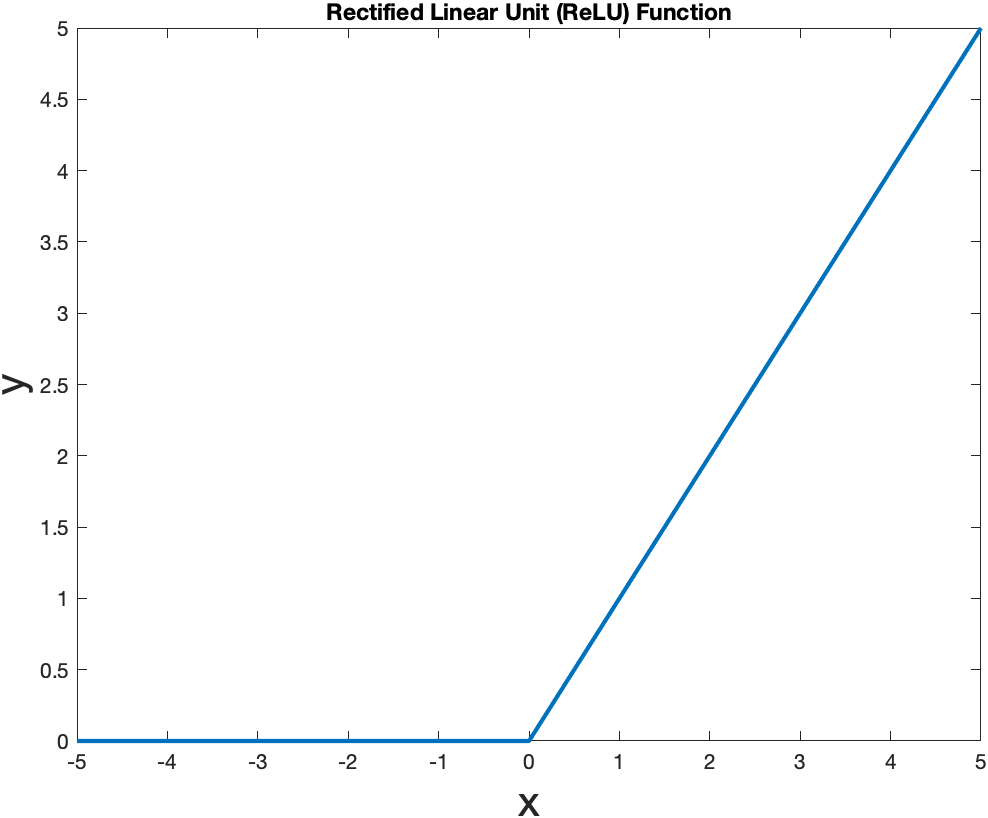
\includegraphics[width=\textwidth]{figures/relu}
            \caption{ReLU function}
            \label{fig:relu}
        \end{subfigure}
        \hspace{0.1\textwidth}
        \begin{subfigure}[b]{0.4\textwidth}
            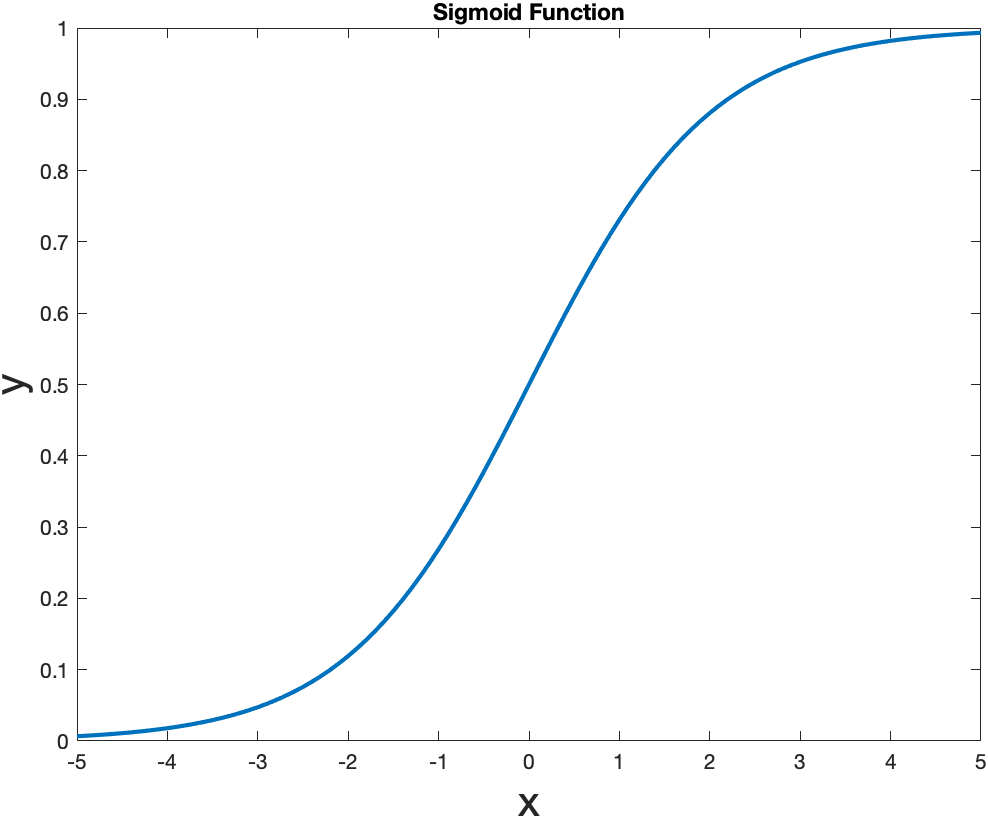
\includegraphics[width=\textwidth]{figures/sigmoid}
            \caption{Sigmoid function}
            \label{fig:sigmoid}
        \end{subfigure}
        \begin{subfigure}[b]{0.4\textwidth}
            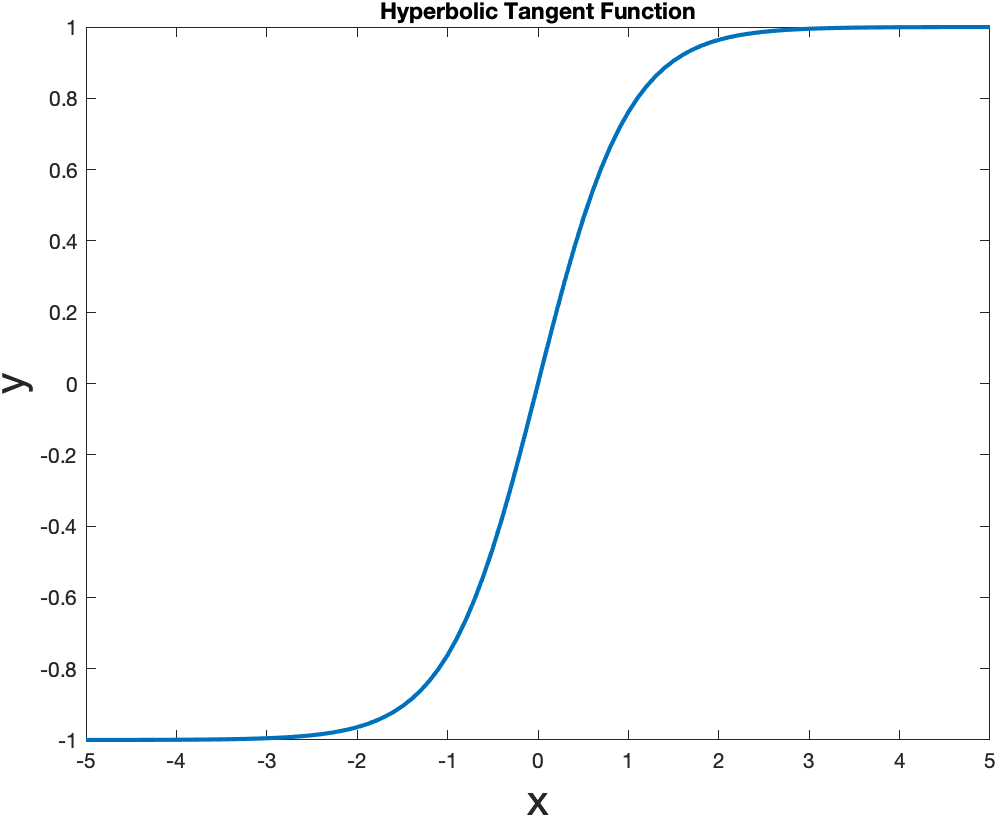
\includegraphics[width=\textwidth]{figures/tanh}
            \caption{Tanh function}
            \label{fig:tahn}
        \end{subfigure}
        \hspace{0.1\textwidth}
        \begin{subfigure}[b]{0.4\textwidth}
            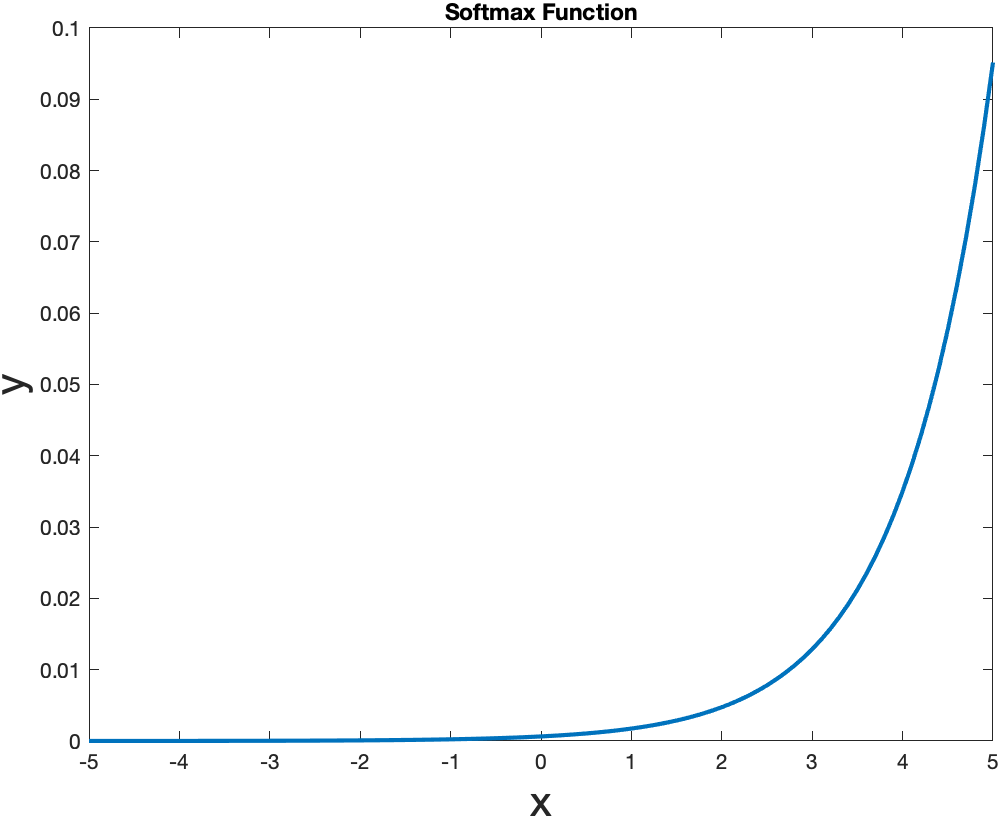
\includegraphics[width=\textwidth]{figures/softmax}
            \caption{Softmax function}
            \label{fig:sigmsoftmaxoid}
        \end{subfigure}
        \begin{subfigure}[b]{0.4\textwidth}
            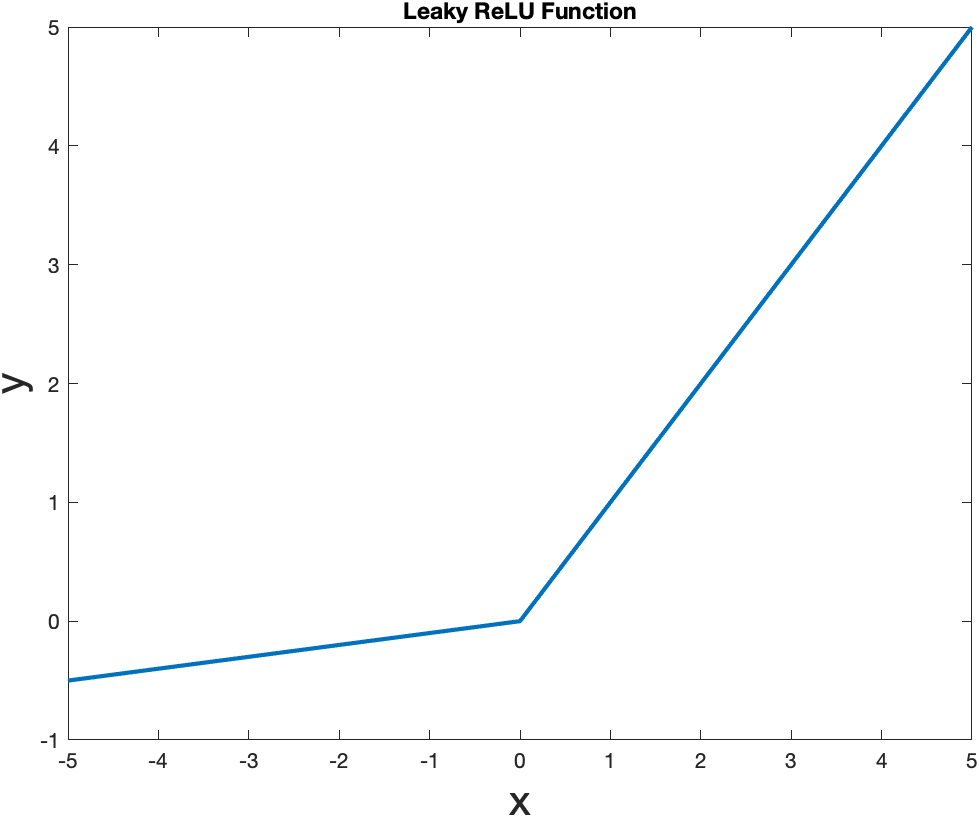
\includegraphics[width=\textwidth]{figures/leakyrelu}
            \caption{Leaky ReLU function}
            \label{fig:leakyrelu}
        \end{subfigure}
        \hspace{0.1\textwidth}
        \begin{subfigure}[b]{0.4\textwidth}
            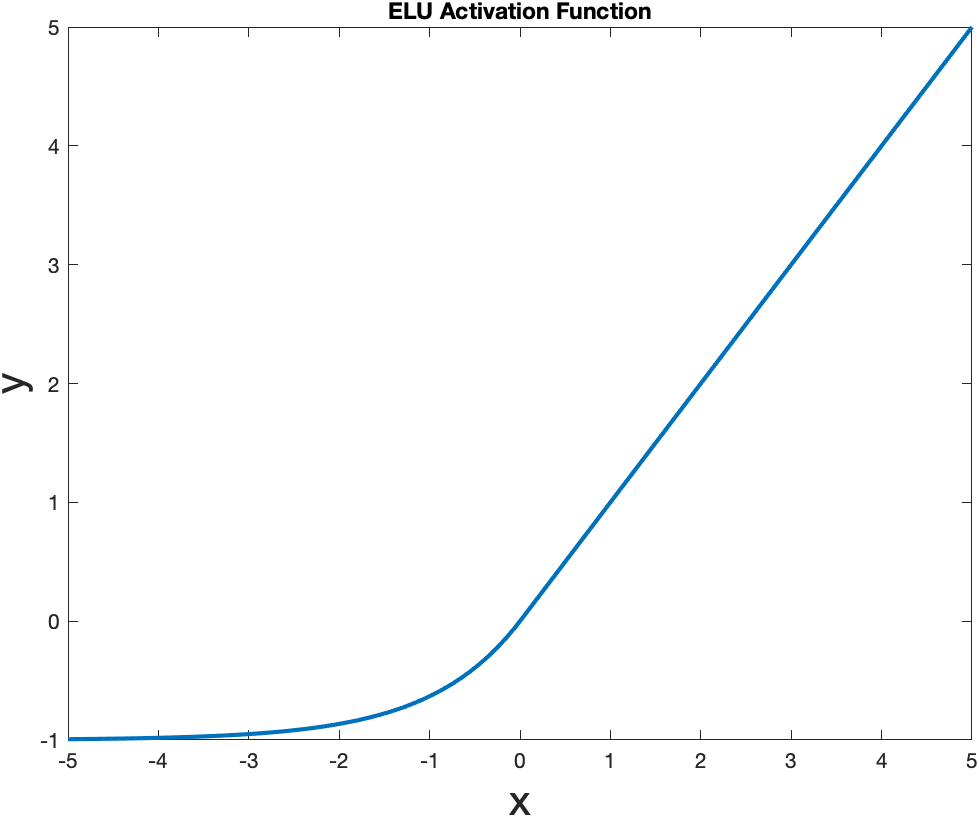
\includegraphics[width=\textwidth]{figures/elu}
            \caption{ELU function}
            \label{fig:elu}
        \end{subfigure}
        \caption{Neural network activation functions.}
        \label{fig:activationfunctions}
    \end{figure}

    \subsection{Application of neural netwrok in prediction} \label{subsec:nnprediction}
    Neural networks can be used for long-term linear prediction in time-series data, including speech, health, and stock data. Neural networks can be trained to model and forecast the~patterns in the~data, including shifts in the long-term linear prediction. Neural networks have been shown to be effective in capturing the~complex relationships between variables in time-series data, and can learn to identify subtle patterns and trends that may be difficult to detect using traditional statistical methods. In the~context of long-term linear prediction, neural networks can be trained on historical data to identify prev    atterns and trends in the~data and make predictions for future values.\\
    \\
    They can also be used to detect shifts in the~long-term linear prediction, which can be useful for identifying changes in the~underlying processes that generate the~data. However, it's important to note that neural networks can be computationally expensive and require large amounts of data to train effectively. They also require careful tuning of hyperparameters and selection of appropriate architecture to achieve good performance. In addition, the~interpretation of the~results of a~neural network can be more challenging than with traditional statistical methods. Overall, neural networks can be a~powerful tool for long-term linear prediction in time-series data, including shifts in the~data, but their use should be carefully considered based on the~specific application and available data.
    \\
    \chapter{Implementation}
      Let's prepare the application which will be used all principles describes in~\ref{analysis}. Created project is focused on the design and development of the Automatic prediction model builder system in the form of an application with a user-friendly user interface, which will be implemented in the cloud environment. As a development environment Matlab ecosystem was used.
        \section{Mathematical models}
        Prediction models were based mainly on the principle of linear prediction (LP) and its modifications, such as non-integer linear prediction (fractional linear prediction - FLP), LP extended by parameters capable of capturing short-term and long-term trendiness in data (extended linear prediction - ELP), etc., which will be extended by further statistical methods such as Monte Carlo, Markov chains, etc.\\
        \\
        For the identification of the appropriate structure of economic and behavioral models and the identification of the parameters of the selected models, machine learning algorithms will be used, which will provide the optimal solution for the selected data and thus the use-case.
        \section{Application overview}
        This application would make it possible to easily and accurately predict various socioeconomic macro and micro indicators, such as gross/net domestic/national product, economic wealth, unemployment, inflation, average/minimum wage, purchasing power of the population but also the behavior of customers (customers can also be perceived as households), intended for sectors such as public or state administration, public planning (but also private) finance, banking.\\
        \\
        From the point of view of commercial use, a possible application would be predicting the number of customers and the number of orders, the company's income, the success of marketing strategies, or on the basis of the prediction, the planning of warehouse stocks.
        \section{Data identification}
        \section{User Interface}
        \section{Test cases}
        

\end{document}


\subsection{Regression models}\label{sec:regression}
